\chapter{Walidacja rozwiązania}
\label{cha:tests}
Po wstępnym nastrojeniu układu, należy uruchomić oraz przetestować urządzenie. Autor zapoznał się w~tym celu z~normą dotyczącą mierzenia poziomu natężenia hałasu \cite{test_norm}, jednak ze względów subiektywnych nie zastosował się do niej, a~obrał własną metodę wykonania testu. Ze względu na niskie amplitudy sygnałów występujących w~urządzeniu i~podczas testu, autor zdecydował się przetestować urządzenie akwirując sygnały przy użyciu oscyloskopu. Zarówno sposób, jak i~wyniki pomiarów, opisane są w~sekcji \ref{sec:practical_test}.
\section{Typowe rodzaje hałasu}
Jak już wspomniano w~sekcji \ref{sec:hałas} rozdziału \ref{cha:teoria}, typowymi rodzajami hałasu, które można chcieć tłumić takim urządzeniem, są:
\begin{itemize}
	\item rozmowy pobliskich osób,
	\item szum wentylacyjny,
	\item dźwięk towarzyszący pracy silnika.
\end{itemize}
Są to zatem sygnały charakteryzujące się (w~przybliżeniu) stałym przedziałem częstotliwościowym i~niewielkim natężeniem, jednak będące uciążliwymi w~dłuższej perspektywie czasowej. W~ramach testu praktycznego sprawdzono działanie układu przy ekspozycji na hałas pochodzący od sygnałów sinusoidalnych, złożeń kilku takich sygnałów (np. sygnał sinusoidalny o~częstotliwości \SI{200}{\Hz} + \SI{700}{\Hz}), sygnałów prostokątnych oraz użyto sygnału z~wobulatora (będący ,,przemieceniem" wszystkich częstotliwości w~zakresie pracy filtra), aby sprawdzić wpływ przegrody dźwiękochłonnej na pracę układu.
\section{Test praktyczny}
\label{sec:practical_test}
\subsection{Warunki testu}
\label{subsec:circumstances}
Układ został przetestowany w~pomieszczeniu przeznaczonym dla prowadzenia zajęć laboratoryjnych. W~trakcie przeprowadzania testu nie występowały inne, znaczące źródła hałasu, które mogłyby w~niekontrolowany sposób zakłócać pracę układu i~pomiar. Do akwizycji sygnałów obecnych bezpośrednio na~połączeniach układu zastosowano oscyloskop cyfrowy, w~którym wykorzystano 3~kanały pomiarowe. Kanał pierwszy podłączono do sygnału mikrofonu głównego, aby zmierzyć poziom hałasu bez tłumienia. Kanał drugi oscyloskopu podłączony został do sygnału pochodzącego z~mikrofonu odsłuchowego, zaś ostatni z~kanałów użyty został do zmierzenia napięć obecnych na połączeniu wyjścia przetwornika C/A. Pozwoliło to na bezpośredni i~jednoczesny podgląd trzech kluczowych zmiennych. W~zależności od potrzeby, włączano lub wyłączano algorytm i~w~obu przypadkach zapisywano dane pochodzące z~urządzenia pomiarowego celem opracowania ich na komputerze~PC.

Głośnik użyty do odgrywania dźwięków podłączono do generatora funkcyjnego i~umieszczono go w~bliskiej odległości od mikrofonu głównego zbudowanego urządzenia. Odległość od źródła dźwięku wynosiła \SI{45}{\mm}, zaś czas pomiaru był zmienny dla każdego z~etapów, co wynika bezpośrednio z~ilości czasu, jaką zajmuje strojenie filtra dla bardziej złożonych sygnałów. Ostatecznie, w~ramach każdego etapu testu, czekano aż filtr nastroi się względem podawanego hałasu, by następnie zapisać dane z~oscyloskopu cyfrowego.
\subsection{Wyniki testów}
Celem sprawdzenia jakości zbudowanego urządzenia, dokonano testu praktycznego, gdzie w~pomieszczeniu laboratoryjnym zmierzono poziom natężenia hałasu słyszanego przez mikrofony urządzenia. Do generowania dźwięków testowych użyto głośnika podłączonego do generatora funkcyjnego. Łącznie dokonano siedmiu pomiarów z~akwizycją sygnału w~trzech wariantach -- bez tłumienia, tylko z~tłumieniem pasywnym, oraz z~tłumieniem pasywnym i~uruchomionym tłumieniem aktywnym pochodzącym z~zaprogramowanego układu. Podczas testów tłumienia aktywnego, po pewnym czasie działania i~uczenia algorytmu, odczytywano wagi filtra LMS, co pozwoliło wyznaczyć jego odpowiedź impulsową.

Należy przypomnieć, że celem zamodelowania nieidealnego przylegania słuchawek do głowy użytkownika, zastosowano element dystansowy w~postaci długopisu, rozdzielający muszle nauszników. Powoduje to lekkie zwiększenie poziomu natężenia hałasu, jaki dociera do mikrofonu odsłuchowego oraz uwydatnia działanie aktywnej części projektu autora. 
Podczas przeprowadzania testu, doświadczalnie wyznaczono, że efektywnym zakresem aktywnego tłumienia hałasu jest pasmo częstotliwościowe od około \SI{400}{\Hz} do około \SI{820}{\Hz}. Okazuje się, że poniżej dolnej granicy pasma, do głosu zaczynają dochodzić nieliniowości zawieszenia membrany głośnika oraz jego częstotliwości rezonansowe. Można częściowo zmniejszyć wpływ tych czynników na pomiar poprzez zmniejszenie amplitudy podawanego hałasu, wtedy jednak szumy wewnątrz-układowe zaczynają stanowić znaczącą część sygnału. Niewykluczone również, że kształt i~rozmiar przestrzeni wewnątrz muszli użytej słuchawki może powodować powstawanie fal stojących, gdzie dla pewnych częstotliwości mikrofon odsłuchowy mógłby się znaleźć w~strzałce lub węźle --  a~to wpływałoby znacznie na odczytywane wartości i~powodowałoby rozstrojenie filtra. Z~kolei powyżej górnej granicy pasma aktywne tłumienie traciło swą efektywność na rzecz tłumienia pasywnego. Choć można było próbować dokonywać pomiarów dla wyższych częstotliwości hałasu, to autor w~chwili testu nie dysponował przyrządami pomiarowymi o~wyższej dokładności i~mniejszym zaszumieniu. Z~tych powodów uznano, że wymieniony zakres będzie odpowiednio dobrym punktem startowym urządzenia, gdzie można już zauważyć efekty działania projektu, jednak wciąż pozostaje dużo możliwości jego poprawy.

W~związku z~takimi możliwościami prototypu, dokonano następujących siedmiu pomiarów:
\begin{enumerate}
	\item Test sinusoidy o~częstotliwości równej \SI{400}{\Hz}, amplitudzie równej 3~Vpp. (rys. \ref{fig:test_1_off}, \ref{fig:test_1_on})\\
	\begin{figure}[h!]
		\centering
		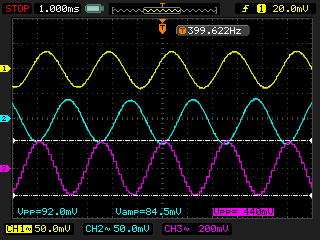
\includegraphics[scale=0.7]{../Assets/Results/1_400_3_off.png}
		\caption{Przebieg sygnałów przy wyłączonym algorytmie dla pomiaru~1.}
		\label{fig:test_1_off}
	\end{figure}
	\begin{figure}[h!]
		\centering
		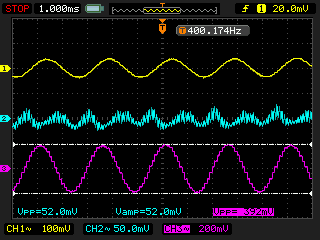
\includegraphics[scale=0.7]{../Assets/Results/1_400_3_on.png}
		\caption{Przebieg sygnałów przy włączonym algorytmie dla pomiaru~1.}
		\label{fig:test_1_on}
	\end{figure}
	W~pierwszym pomiarze sprawdzono charakter pracy urządzenia dla częstotliwości z~dolnych granic możliwości 
	\item Test sinusoidy o~częstotliwości równej \SI{579}{\Hz}, amplitudzie równej 5~Vpp.\\
	\begin{figure}[h!]
		\centering
		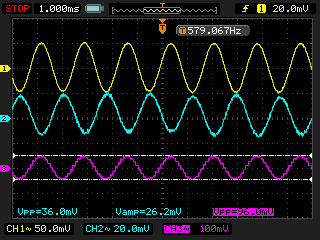
\includegraphics[scale=0.7]{../Assets/Results/2_579_5_off.png}
		\caption{Przebieg sygnałów przy wyłączonym algorytmie dla pomiaru~2.}
		\label{fig:test_2_off}
	\end{figure}
	\begin{figure}[h!]
		\centering
		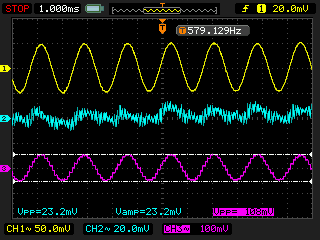
\includegraphics[scale=0.7]{../Assets/Results/2_579_5_on.png}
		\caption{Przebieg sygnałów przy włączonym algorytmie dla pomiaru~2.}
		\label{fig:test_2_on}
	\end{figure}
	\item Test sinusoidy o~częstotliwości równej \SI{820}{\Hz}, amplitudzie równej 8~Vpp.\\
	\begin{figure}[h!]
		\centering
		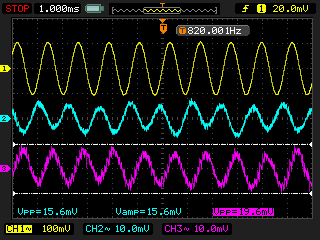
\includegraphics[scale=0.7]{../Assets/Results/3_820_8_off.png}
		\caption{Przebieg sygnałów przy wyłączonym algorytmie dla pomiaru~3.}
		\label{fig:test_3_off}
	\end{figure}
	\begin{figure}[h!]
		\centering
		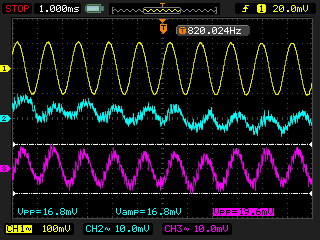
\includegraphics[scale=0.7]{../Assets/Results/3_820_8_on.png}
		\caption{Przebieg sygnałów przy włączonym algorytmie dla pomiaru~3.}
		\label{fig:test_3_on}
	\end{figure}
	\item Test sinusoidy o~częstotliwości równej \SI{250}{\Hz}, amplitudzie równej 6~Vpp.\\
	\begin{figure}[h!]
		\centering
		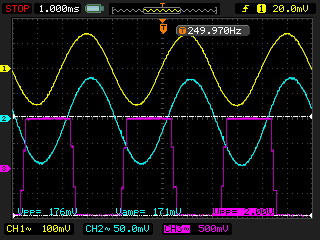
\includegraphics[scale=0.7]{../Assets/Results/4_250_6_off.png}
		\caption{Przebieg sygnałów przy wyłączonym algorytmie dla pomiaru~4.}
		\label{fig:test_4_off}
	\end{figure}
	\begin{figure}[h!]
		\centering
		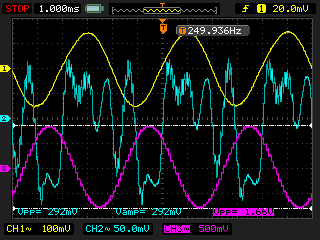
\includegraphics[scale=0.7]{../Assets/Results/4_250_6_on_notworking.png}
		\caption{Przebieg sygnałów przy włączonym algorytmie dla pomiaru~4.}
		\label{fig:test_4_on}
	\end{figure}	
	\item Test sygnału prostokątnego o~częstotliwości równej \SI{720}{\Hz}, amplitudzie równej 3~Vpp.\\
	\begin{figure}[h!]
		\centering
		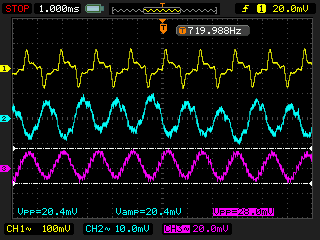
\includegraphics[scale=0.7]{../Assets/Results/5_720_3_sq_off.png}
		\caption{Przebieg sygnałów przy wyłączonym algorytmie dla pomiaru~5.}
		\label{fig:test_5_off}
	\end{figure}
	\begin{figure}[h!]
		\centering
		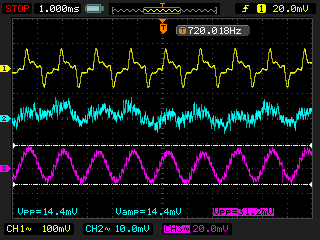
\includegraphics[scale=0.7]{../Assets/Results/5_720_3_sq_on.png}
		\caption{Przebieg sygnałów przy włączonym algorytmie dla pomiaru~5.}
		\label{fig:test_5_on}
	\end{figure}	
	\begin{figure}[h!]
		\centering
		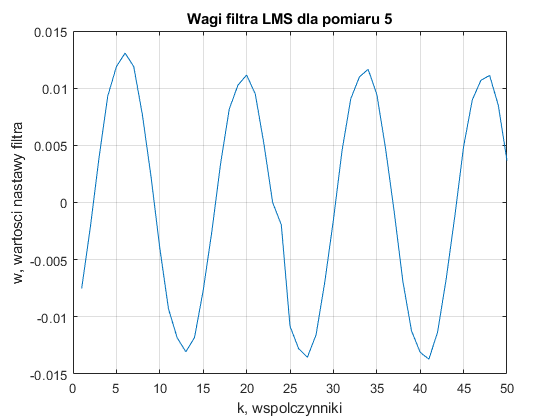
\includegraphics[scale=0.7]{../Assets/Results/5_wagi_lms.png}
		\caption{Odpowiedź impulsowa filtra dla pomiaru~5.}
		\label{fig:test_5_lms}
	\end{figure}
	\item Test sygnału złożonego z~sinusoidy 1~o~częstotliwości równej \SI{451}{\Hz}, amplitudzie równej 3,1~Vpp oraz sinusoidy 2~o~częstotliwości \SI{627}{\Hz}, amplitudzie równej 6,6~Vpp.\\
	\begin{figure}[h!]
		\centering
		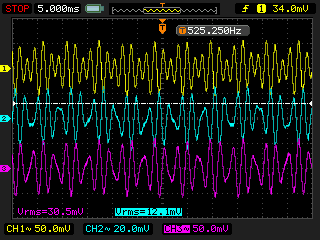
\includegraphics[scale=0.7]{../Assets/Results/6_complex_off.png}
		\caption{Przebieg sygnałów przy wyłączonym algorytmie dla pomiaru~6.}
		\label{fig:test_6_off}
	\end{figure}	
	\begin{figure}[h!]
		\centering
		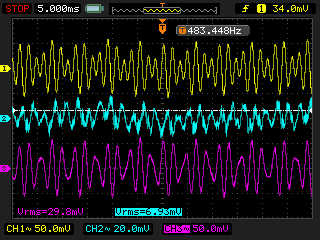
\includegraphics[scale=0.7]{../Assets/Results/6_complex_on.png}
		\caption{Przebieg sygnałów przy włączonym algorytmie dla pomiaru~6.}
		\label{fig:test_6_on}
	\end{figure}
	\begin{figure}[h!]
		\centering
		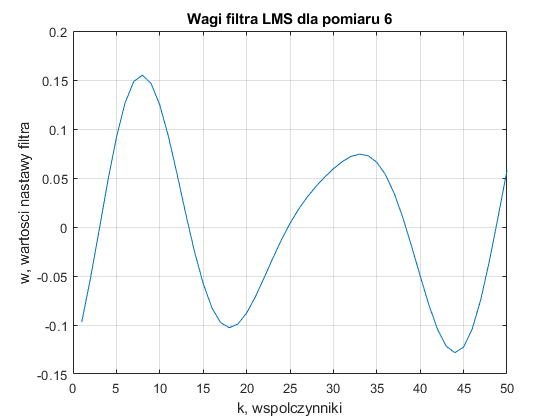
\includegraphics[scale=0.7]{../Assets/Results/6_wagi_lms.png}
		\caption{Odpowiedź impulsowa filtra dla pomiaru~6.}
		\label{fig:test_6_lms}
\end{figure}
	\item Test sygnału ,,sweep'' przy wyłączonym algorytmie.\\
	Ostatni z~testów miał na celu wyznaczenie charakterystyki Bodego pasywnej osłony dźwiękochłonnej użytej w~projekcie. ,,Przemiatano'' częstotliwości w~zakresie efektywnego tłumienia urządzenia, jednak przy wyłączonym algorytmie. W~tym teście głównym celem było ukazanie faktycznych różnic w~zastosowaniu pasywnego oraz aktywnego tłumienia. Wyznaczona w~ten sposób charakterystyka znajduje się na rysunku \ref{fig:bode}.
	\begin{figure}[h!]
		\centering
		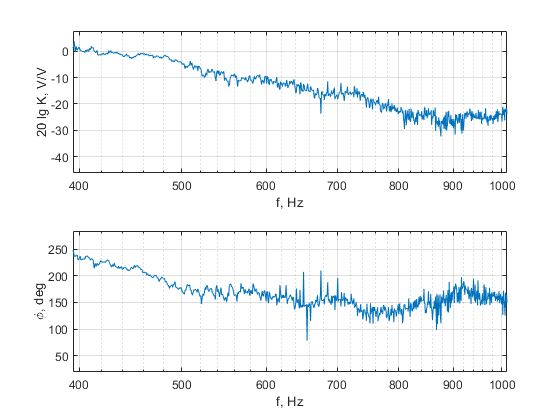
\includegraphics[scale=0.9]{../Assets/bode_przegrode.png}
		\caption{Charakterystyka Bodego przegrody dźwiękochłonnej.}
		\label{fig:bode}
	\end{figure}

Zgodnie z~omawianymi w~rozdziale \ref{cha:teoria} różnicami, na wspomnianej charakterystyce można zauważyć, że skuteczność tłumienia nauszników pasywnych wzrasta razem z~częstotliwością sygnału do wytłumienia. Aby osadzić pionową oś charakterystyki amplitudowej, porównano napięcie przesyłane przez mikrofon feedforward z~napięciem pochodzącym z~mikrofonu feedback. Wykres ten przedstawiony jest tutaj głównie jako ciekawy dodatek i~wyjaśnienie kwestii pasywnej. Pozostaje on jednak do dalszego zgłębienia, bowiem pomimo faktu, iż autor nie potrzebował znać dokładnych parametrów przegrody w~tym projekcie, to znajomość tej charakterystyki może być przydatna w~dalszych iteracjach i~usprawnieniach urządzenia.
\end{enumerate}

\subsection{Poziom hałasu bez tłumienia}
Pomiaru bez tłumienia dokonano poprzez akwizycję sygnału z~mikrofonu głównego (feedforward). Pozwoliło to na zebranie danych o~poziomie natężenia hałasu przed jego przejściem przez osłonę dźwiękoszczelną. Przy założeniu opisanych w~sekcji \ref{subsec:circumstances} warunków testu, średni poziom hałasu zmierzony bez żadnego sposobu tłumienia wyniósł PLACEHOLDER. %TODO uzupełnić pomiar.
Widmo częstotliwościowe pokazano na rysunku \ref{fig:widmo_bez}.


\subsection{Poziom hałasu z pasywnym tłumieniem}
Następnie, aby dokonać pomiaru natężenia hałasu przy pasywnym tłumieniu, zamknięto i~zebrano dane pochodzące z~drugiego mikrofonu (feedback). Dzięki temu otrzymano informację o~tym, jaki poziom hałasu panuje wewnątrz słuchawki, czyli jaki hałas słyszałby użytkownik przy użyciu jedynie pasywnego tłumienia, które dają użyte nauszniki. Należy pamiętać, że zmieni się w~ten sposób również odległość od źródła hałasu do mikrofonu pomiarowego. Różnicę tę można jednak zawrzeć w~efektach działania tłumienia pasywnego -- odległość od źródła dźwięku również jest jedną ze składowych podejścia pasywnego. Przy tych samych założeniach, średni poziom hałasu wyniósł PLACEHOLDER2. %TODO uzupełnić pomiar.
Widmo częstotliwościowe zaprezentowano na rysunku \ref{fig:widmo_pasywnie}. 


Dodatkowo, porównując wynik pomiaru bez tłumienia hałasu z~wynikiem otrzymanym w~tej sekcji, można wyznaczyć charakterystykę częstotliwościową osłony dźwiękoszczelnej. Aby informacja była miarodajna, należy posłużyć się do tego celu wobulatorem, który zapewnia sygnał dźwiękowy o~narastającej częstotliwości i~stałej amplitudzie. Taki rodzaj sygnału ujawnia szerokość pasma, które efektywnie tłumione jest przez samą osłonę o~wysokim współczynniku tłumienia. Wynik pomiaru, umieszczony na rysunku \ref{fig:sweep} pozwala lepiej zapoznać się z~parametrami akustycznymi użytych słuchawek i~w~dalszych iteracjach projektu usprawnić strojenie algorytmu tak, aby pasował do tego typu słuchawek.

\subsection{Poziom hałasu z aktywnym tłumieniem}
Ostatecznie, aby dowieść skuteczności rozwiązania, uruchomiono algorytm i~ponownie zebrano dane z~mikrofonu odsłuchowego. Średni poziom hałasu zmierzony w~ten sposób wyniósł PLACEHOLDER3. %TODO uzupełnić pomiar.
Widmo częstotliwościowe zamieszczono na rysunku \ref{fig:widmo_aktywnie}.


Na końcu tak wykonanego pomiaru odczytano wartości wag filtra LMS. Te nastawy zostały osiągnięte przez filtr w~całości samodzielnie, gdyż nie ustawiano żadnych wartości początkowych -- filtr był zerowany przy każdorazowym uruchomieniu. Taki pomiar pozwala na wyznaczenie odpowiedzi impulsowej zastosowanego filtra. Wizualizacja tych danych w~pakiecie obliczeniowym MATLAB pozwala na lepsze zrozumienie zachowania oraz możliwości adaptacyjnych filtra.
%TODO mikrofon z peceta do przestrzeni, zmierzyc widmo dzwieku do matlaba